% Yeban User Guide — Chapter 3: Tracks and Clips (English)
% T-DOC-001 chapter-by-chapter delivery, written ahead of the CH03 task.
% Sources: app.slint menus and clip-drag callbacks, cli.rs SHORTCUTS, docs/manual/01-overview.md.

\chapter{Tracks and Clips}
\label{ch:tracks-clips}

\begin{quote}
方以类聚，物以群分。
\end{quote}

Source: Book of Changes, “Appended Judgments I” (《周易·系辞上》). Translation: “Things gather according to their kind; creatures divide according to their group.”

Tracks and clips find their place by kind; clear grouping is what makes editing orderly.

The arrangement area is Yeban's main workspace: tracks as rows, clips laid out on the
timeline to their right. This chapter covers creating tracks, placing clips and turning
a piece of material into the arrangement you want.

\section{Track Types and the Track Header}

\subsection{Three track types}

The Track menu offers three creation entries:

\begin{itemize}
  \item \textbf{New MIDI Synth Track (Cmd/Ctrl+N)}: sounds via a built-in synthesizer or plugin instrument, holding MIDI clips.
  \item \textbf{New Audio Track}: holds recorded or imported audio clips.
  \item \textbf{New Aux Bus Track}: receives sends from other tracks for summing and group processing.
\end{itemize}

Delete Selected Track removes the selected track from the menu.

\subsection{The track header}

Each track's left side is the header: name, mute/solo switches, volume, and the Track
Menu button at the very front (collecting that track's operations). Mute silences the
track; solo listens only to it; both can also be operated in the mixer console
(Chapter 7).

\screenshot{ch03-track-header}{Close-up of a track header labelling the Track Menu button, name, mute/solo and volume}

\section{Create, Move, Copy and Split Clips}

\subsection{Create a clip}

Once a clip is created on a track it appears on the timeline. Its content depends on
the track type: notes on a MIDI track (written in the piano roll, Chapter 4), audio
material on an audio track. An empty MIDI clip defaults to four bars, its tick length
derived from the project's time signature; if the time signature is invalid the app
reports ``invalid time signature, cannot compute clip length'' instead of inventing
a length.

\subsection{Move, resize and cut/copy/paste}

\begin{itemize}
  \item \textbf{Move}: drag to reposition; drag either edge to resize.
  \item \textbf{Copy / Paste / Cut}: Cmd/Ctrl+C, Cmd/Ctrl+V, Cmd/Ctrl+X, matching the Edit menu group.
  \item \textbf{Split}: select a clip and press Cmd/Ctrl+T to cut it at the playhead.
\end{itemize}

Dragging previews the destination before you release; you can cancel mid-drag without
leaving a half-finished state.

\begin{figure}[htbp]
\centering
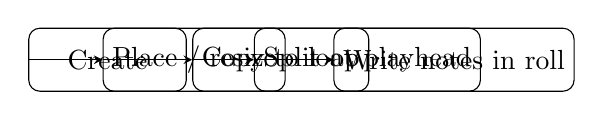
\begin{tikzpicture}[node distance=1.1cm, >=stealth,
    box/.style={draw, rounded corners, align=center, minimum width=2.0cm, minimum height=0.8cm}]
  \node[box] (a) {Create};
  \node[box, right of=a] (b) {Place / resize};
  \node[box, right of=b] (c) {Copy to loop};
  \node[box, right of=c] (d) {Split at playhead};
  \node[box, right of=d] (e) {Write notes in roll};
  \draw[->] (a)--(b); \draw[->] (b)--(c); \draw[->] (c)--(d); \draw[->] (d)--(e);
\end{tikzpicture}
\caption{Common clip flow: create $\to$ place $\to$ copy $\to$ split $\to$ write notes}
\label{fig:ch03-clip-flow}
\end{figure}

\section{Stretch, Merge and Multi-select Editing}

Dragging a clip's edge changes only its time span, not the pitch or relative timing of
its notes (for audio, it changes the playback range). To join adjacent clips into one
continuous piece, align their boundaries first, then merge; the two clips become one
and undo restores them.

With several clips selected, copy, cut and delete apply to the whole group. If only
part of a group is selected, the operation follows the selection and does not touch
unselected clips.

\screenshot{ch03-multi-select}{Three clips selected in the arrangement area with a group-drag preview}

\section{Clip Parameters and the Clip Launch Matrix}

Selecting a clip shows its identity (name, owning track) and editable parameters in
the inspector/clip parameter area. Press Tab to open the \textbf{Clip Launch Matrix}
(Session view): the interface becomes a grid of clips; click a cell to fire that clip,
which suits live launching and improvised arrangements. F5 also switches to Session
view; F6 returns to the Arrangement view.

\screenshot{ch03-clip-matrix}{The Clip Launch Matrix with cells arranged by track, one cell firing}

\section{Cross-track Drag and Track Change}

In the current version, dragging a clip changes only its horizontal position within
the same track. Moving a clip from one track to another is still in evolution
(work item T-FIX-209). So do not treat ``drag onto another track'' as available: to
place material on another track, copy/paste it onto the target track and delete the
original until the capability officially lands. Yeban does not disguise an
unimplemented operation as a success.

\section{Help Topic Mapping}

\begin{table}[htbp]
\centering
\caption{Sections of this chapter $\to$ in-app help anchors}
\label{tab:ch03-help}
\begin{tabular}{ll}
\hline
Section & Help topic \\
\hline
Track types / track header & \texttt{tracks-types-header} \\
Create clips & \texttt{clips-create} \\
Move, resize, cut/copy/paste & \texttt{clips-move-resize} \\
Merge and multi-select editing & \texttt{clips-merge-multiselect} \\
Clip parameters / launch matrix & \texttt{clips-launch-matrix} \\
Cross-track drag and track change & \texttt{clips-cross-track} \\
\hline
\end{tabular}
\end{table}

\paragraph{What you will be able to do} Create the three track types, lay out and cut clips, fire clips from the Launch Matrix, and know which cross-track operations are not yet available.

\paragraph{Hands-on exercise} Create a MIDI synth track and an audio track; create a four-bar MIDI clip, copy it into a two-bar loop and split it at the playhead with Cmd/Ctrl+T; press Tab for Session view and fire a cell; press F6 to return to Arrangement and verify the clips are still there.
